\documentclass[twocolumn,prl,aps,superscriptaddress
               ,footinbib,amsfonts,amsmath,amssymb,showpacs]{revtex4-1}

\usepackage[T1]{fontenc}
\usepackage{blindtext}

\usepackage{graphics,graphicx}% Include figure files
\usepackage{dcolumn}% Align table columns on decimal point
\usepackage{bm}% bold math
\usepackage{epsfig}
\usepackage[usenames]{color}
\usepackage{hyperref} 
%\usepackage{showkeys}
\usepackage{mathbbol}
\usepackage{epstopdf}
\usepackage{simplewick}
\usepackage[utf8]{inputenc} 
\usepackage{slashed}
\usepackage{soul}
\usepackage[dvipsnames]{xcolor}


% short-hands
\def\Phperp{P_{h\perp}}
\def\kT{k_T}
\def\pperp{p_\perp}
\def\bfPhperp{{\bm P}_{h\perp}}
\def\bfkT{{\bm k}_T}
\def\bfpperp{{\bm p}_\perp}
\def\avPhperp{\la \Phperp^2 \ra}
\def\avkT{\la \kT^2 \ra}
\def\avpperp{\la \pperp^2 \ra}
\def\bfhp{\hat{\bm h}}
\newcommand{\la}{\langle}
\newcommand{\ra}{\rangle}

\newcommand{\rep}[2]{{\color{blue} \st{#1}} {\color{red} #2}}
\newcommand{\red}[1]{{\color{red} {#1}}}
\newcommand{\green}[1]{{\color{PineGreen} {#1}}}
\newcommand{\com}[1]{{\color{red} [\textbf{#1}]}}

\usepackage[normalem]{ulem}
\newcommand{\old}[1]{{\color{red}\sout{#1}}}
\newcommand{\new}[1]{{\color{blue}#1}}

\begin{document}

%\title{\bf First global analysis of quark-gluon correlations in hadrons from transverse-spin data}
%\title{\bf First global analysis of single transverse-spin asymmetries}
%%% just a suggestion (zhongbo), make it simple/intuitive, not jargon word
%\title{\bf The origin of single transverse-spin asymmetries in hard processes}
%%% Just a suggestion, Alexei
\title{\bf The origin of single transverse-spin asymmetries in high-energy collisions}
%%% A sligh modification, Daniel


\author{Justin Cammarota} 
\affiliation{Department of Physics, 
             College of William and Mary, 
             Williamsburg, Virginia 23187, USA}
\affiliation{Department of Physics, 
             Lebanon Valley College, 
             Annville, Pennsylvania 17003, USA}
%
\author{Leonard Gamberg} 
\affiliation{Division of Science, 
             Penn State University Berks, 
             Reading, Pennsylvania 19610, USA}
%
\author{Zhong-Bo Kang} 
\affiliation{Department of Physics and Astronomy, 
             University of California, 
             Los Angeles, California 90095, USA}
\affiliation{Mani L.~Bhaumik Institute for Theoretical Physics, 
             University of California, 
             Los Angeles, California 90095, USA}
\affiliation{Center for Frontiers in Nuclear Science, 
             Stony Brook University, 
             Stony Brook, New York 11794, USA}             
%
\author{\\ Joshua A. Miller}
\affiliation{Department of Physics, 
             Lebanon Valley College, 
             Annville, Pennsylvania 17003, USA}
%
\author{Daniel Pitonyak}
\affiliation{Department of Physics, 
             Lebanon Valley College, 
             Annville, Pennsylvania 17003, USA}
%
\author{Alexei Prokudin}
\affiliation{Division of Science, 
             Penn State University Berks, 
             Reading, Pennsylvania 19610, USA}
\affiliation{Theory Center, Jefferson Lab, 
             Newport News, Virginia 23606, USA \\
\vspace*{0.2cm}
{\bf Jefferson Lab Angular Momentum (JAM) Collaboration
\vspace*{0.2cm} }}
%
\author{Nobuo Sato}
\affiliation{Theory Center, Jefferson Lab, 
             Newport News, Virginia 23606, USA \\
\vspace*{0.2cm}
{\bf Jefferson Lab Angular Momentum (JAM) Collaboration
\vspace*{0.2cm} }}

\begin{abstract}
\noindent 
%It is believed that the origin of all single transverse-spin
%asymmetries (SSAs) in hard processes isin the intrinsic
%quantum-mechanical interference of multi-parton states that manifest
%itself in eithertwist-3 correlation functions or Transverse Momentum
%Dependent distributions (TMDs). In thispaper, we, for the first time,
%demonstrate that indeed SSAs in hard processes have the same
%origin.We perform the first global analysis of data from
%Semi-Inclusive Deep Inelastic Scattering, Drell-Yan, $e^+e^-$
%annihilation in hadron pairs, and proton-proton scattering and
%extract a unique set offunctions that describe all data.
In this letter, we present, for the first time, a phenomenological
analysis that shows all single transverse-spin asymmetries (SSAs) in
high-energy collisions have the same origin.  
Namely, they are due to the intrinsic quantum-mechanical interference
of multi-parton states.
We perform the first global fit of SSA data from  Semi-Inclusive Deep
Inelastic Scattering, Drell-Yan, $e^+e^-$ annihilation into hadron
pairs, and proton-proton scattering.
Consequently, we are able to identify a unique set of universal 
non-perturbative functions that describe all observed SSAs.
Furthermore, we achieve the first phenomenological agreement with
lattice on the tensor charge of the nucleon.
\end{abstract}

\pacs{}
\maketitle

%%%%%%%%%%%%%%%%%%%%%%%%%%%%%%%%%%%%%%%%%%%%%%%%%%%%%%%%%%%%%%%%%%%%
\noindent {\it \bf Introduction.}
Since the early days of exploring the structure of the nucleon, the
measurements of SSAs posed
certain challenges and puzzles for our understanding of quarks and
gluons as the internal degrees of freedom of the nucleon (generically
called partons), and their dynamics -- see, e.g.,
Refs.~\cite{Bunce:1976yb,Kane:1978nd}. 
%
\green{
Measurements of SSAs in a variety of processes helped to sharpen our
formulation of the underlying theory that describes strong
interactions , \rep{Quantum Chromodynamics (QCD)}{QCD, especially beyond the leading twist}. }
\com{Not sure if this is accurate, certainly other observations have 
done that too which are not SSAs}
%
We departed from the simple picture of a nucleon composed of static
quarks and gluons and developed a more complicated modern picture
where the motion of quarks and gluons, and correlations of their spin
and orbital angular momentum, play a crucial role 
\com{in the observed phenomena?}
-- see, e.g.,
Ref.~\cite{Perdekamp:2015vwa} for a review. 

The intrinsic quantum mechanical correlations of partons in the wave
function of the nucleon, encoded in \red{the} so-called twist-3 functions,
transformed from a rather exotic field of study into the mainstream of
spin physics. 
%
\green{
It was determined that twist-3 functions are the mere reason some SSAs
exist~\cite{Efremov:1981sh, Efremov:1984ip, Qiu:1991pp, Qiu:1998ia,
Kouvaris:2006zy, Eguchi:2006mc, Koike:2009ge, Metz:2012ct,
Kanazawa:2013uia, Beppu:2013uda},
for instance in one-scale reactions like the left-right asymmetry
$A_N$ in proton-proton scattering. 
}
%, and corresponding QCD factorization theorems were developed. 
\com{Determined or, hypothesized? How about this $\to$}
{\color{red}
Many theoretical developments 
~\cite{Efremov:1981sh, Efremov:1984ip, Qiu:1991pp, Qiu:1998ia,
Kouvaris:2006zy, Eguchi:2006mc, Koike:2009ge, Metz:2012ct,
Kanazawa:2013uia, Beppu:2013uda}
indicated that such twist-3 correlation functions 
can exist and be responsible 
for instance in one-scale reactions like the left-right asymmetry
$A_N$ in proton-proton scattering. 
}





Transverse motion of quarks and gluons, encoded into the so-called
Transverse Momentum Dependent (TMD) parton distribution functions
(PDFs) and fragmentation functions (FFs), collectively called TMDs,
were found to be the origin of SSAs in processes where two distinct
scales are measured, such as Semi-Inclusive Deep Inelastic Scattering
(SIDIS) $e\,N^\uparrow \to e\,h\,X$, Drell-Yan (DY) processes
$p^\uparrow \,p \to \ell^+\ell^-\, X$, 
and $e^+e^-$ annihilation into almost back-to-back hadrons (SIA) 
$e^+e^- \to h_1\,h_2\,X$
~\cite{Mulders:1995dh, Boer:1997mf, Bacchetta:2006tn,Arnold:2008kf, Pitonyak:2013dsu}.
%
The corresponding factorization theorems were developed -- see, e.g.,
Refs.~\cite{Collins:2011zzd,GarciaEchevarria:2011rb}.  
%
It was also shown that the twist-3 and TMD formalisms agree in the
momentum region where both are
valid~\cite{Ji:2006br, Koike:2007dg, Ji:2006ub,Yuan:2009dw,Zhou:2008fb,Zhou:2009jm}, thus theoretically establishing a common origin of SSAs. 

New experimental facilities that intend to study hadronic structure
are being started or planned, such as the Jefferson Lab 12 GeV upgrade
or future Electron Ion Collider.
%
Yet, we still lack a phenomenological demonstration that all SSAs
arise from a universal mechanism. 
%
There are many papers dedicated to the description of SSAs using the
TMD formalism or twist-3 formalism separately.  
%
However, it has never been shown that a unique set of functions can
describe all SSAs in SIDIS, DY, $e^+e^-$, and proton-proton
collisions. 

%%%%%%%%%%%


\new{Many theoretical developments~\cite{Efremov:1981sh, Efremov:1984ip, Qiu:1991pp, Qiu:1998ia,Kouvaris:2006zy, Eguchi:2006mc, Koike:2009ge, Metz:2012ct,Kanazawa:2013uia, Beppu:2013uda} indicated that correlations of multi-parton states in the wave function of the nucleon encoded in the twist-3 functions 
 exist and give rise to spin asymmetries in one scale processes, such as left-right asymmetry $A_N$ observed in $p^\uparrow p \to \pi X$. Correlations of multi-parton states in the wave function of the nucleon encoded in the twist-3 functions are believed to give rise to spin asymmetries in one scale processes, such as left-right asymmetry $A_N$ observed in $p^\uparrow p \to \pi X$.
The transverse momentum of the pion  measured in this process sets the scale and makes collinear twist-3 factorization appropriate for description of the asymmetries. On the other hand, in processes, where two different scales are observed, $Q_1 \ll Q_2$, such as SIDIS, DY, $e^+e^-$, a different type of factorization, TMD factorization is 
 appropriate and TMD functions give rise to asymmetries. Nonetheless, in TMD formalism that stems from the original  Collins-Soper-Sterman (CSS)
formalism~\cite{Collins:2011zzd}, the multi-parton collinear correlations play an important role. A generic TMD PDF $F(x,k_T)$ depends on $x$, the longitudinal
momentum fraction of the nucleon's momentum carried by the parton, and $k_T\equiv |\vec{k}_T|$ its
transverse momentum. In Fourier conjugate position space, $b_T$, TMD becomes $\tilde F(x,b_T)$. When $b_T$ (GeV$^{-1}$) is becoming very small it sets a dynamic scale $\propto 1/b_T$ that can be used for Operator Product Expansion of polarised TMDs in terms of multi-parton correlation functions. The other way to establish the  connection is to use the amplitude level relations in the limit of $b_T\to 0$, that result in relations of twist-3 and TMDs such as $\pi F_{FT}(x,x)=f_{1T}^{\perp(1)}(x)$~\cite{Boer:2003cm}, where $F_{FT}(x,x)$ is the so-called Qiu-Sterman matrix element, and $f_{1T}^{\perp(1)}(x)$ is the first moment of Sivers function. The dependence of this relation on the scale is still being debated over. TMDs and twist-3 functions have different divergences that make twist-3 and TMD evolution intrinsically different.

In this letter, we do not address the validity of relations of TMD and twist-3 functions beyond the lowest order, but rather use the lowest order relations of twist-3 functions and TMDs (omitting the full TMD evolution for consistency). We will construct a unique set of twist-3 functions and corresponding TMDs and will attempt description of all available data in pion production in SIDIS, DY, $e^+e^-$, and $p^\uparrow p \to \pi X$. 
}
We will provide, for the first time, a phenomenological
proof based on TMD and twist-3 factorization frameworks that indeed
show that 
the origin of SSAs is universal. We perform a global analysis of the
available measurements in SIDIS, DY, $e^+e^-$, and proton-proton
collisions and extract a unique set of multi-parton correlation
functions that describe all data. As a byproduct of our fit, we
compute the tensor charge of the nucleon and find, for the first time,
an agreement between phenomenology and lattice.




%%%%%%%%%%%%%%%%%%%%%%%%%%%%%%%%%%%%%%%%%%%%%%%%%%%%%%%%%%%%%%%%%%%%
\vspace{0.1cm}
\noindent {\it \bf Theoretical Background.}
%  

\old{Within the current Collins-Soper-Sterman (CSS)
formalism~\cite{Collins:2011zzd} used to study processes like SIDIS,
DY, and SIA, a generic TMD PDF $F(x,k_T)$, with $x$ the longitudinal
momentum fraction of the parton and $k_T\equiv |\vec{k}_T|$ its
transverse momentum, is Fourier transformed to position space $b_T$.
%
This function $\tilde{F}(x,b_T)$ at leading order (LO)}
\com{TMDs are all orders quantity, so I don't understand the meaning of LO}
\old{schematically is written as}~\cite{Collins:2011zzd, Collins:2014jpa,Aybat:2011ge, Bacchetta:2013pqa, Echevarria:2014xaa, Kang:2015msa}
\begin{equation}
\tilde{F}(x,b_T) \sim F_{\rm OPE}(x)\exp[-S_P(b_T)-S^{\tilde{F}}_{NP}(b_T)]\,, 
\label{e:TMD}
\end{equation}
%
\old{where $F_{\rm OPE}(x)$ is a collinear function calculated at small $b_T$
through the operator product expansion (OPE), and $S_P$ and $S_{NP}$
are the so-called perturbative and non-perturbative Sudakov factors,
respectively.
%
The former is universal while the latter depends on the particular
TMD, as emphasized by the superscript.  
%
\green{Note that we have omitted the scale dependence of these functions for
brevity.} \com{can this go into a footnote?} 
%
An analogous formula to (\ref{e:TMD}) can also be written for TMD FFs
$D(z,zp_\perp)$, where $p_\perp$ is the transverse momentum of the
fragmenting parton and $z$ is the momentum fraction carried by the
produced hadron.
}

The most intensely investigated TMD (two-scale) effects over the last
\old{25 years} \new{few decades} have been the Sivers and Collins SSAs in SIDIS, 
$A_{\rm SIDIS}^{\rm Siv}$ 
and 
$A_{\rm SIDIS}^{\rm Col}$; 
Sivers SSA in DY,
$A_{\rm DY}^{\rm Siv}$; 
and Collins SSA in SIA, 
$A_{\rm SIA}^{\rm Col}$.  
The relevant TMDs probed by these processes are the
transversity function $h_1(x,k_T)$, the Sivers function
$f_{1T}^\perp(x,k_T)$, and Collins function
$H_{1}^\perp(z,zp_\perp)$~\cite{Mulders:1995dh, Boer:1997mf,Bacchetta:2006tn, Arnold:2008kf, Pitonyak:2013dsu}.

Each of the above functions \old{can be written in the form~(\ref{e:TMD}),
where,} can be related to its collinear counterpart via OPE, in particular, \old{the OPE piece for} $h_1(x,k_T)$ is \new{related} the collinear
twist-2 transversity function $h_1(x)$~\cite{Bacchetta:2013pqa}; for
$f_{1T}^\perp(x,k_T)$ is the so-called Qiu-Sterman function
$F_{FT}(x,x)$~\cite{Aybat:2011ge}; and for $H_{1}^\perp(z,zp_\perp)$
is its first $p_{\perp}$-moment 
$
H_1^{\perp(1)}(z) 
    \equiv z^2\int d^2 \vec{p}_\perp\,(p_\perp^2/(2M_h))
    H_{1}^\perp(z,zp_\perp)
$
~\cite{Kang:2015msa}, where $M_h$ is the
hadron mass.
%
The functions $F_{FT}(x,x)$ and $H_1^{\perp(1)}(z)$ are
twist-3 and connected to quark-gluon correlations in hadrons.  Note
that one also has 
$
\pi F_{FT}(x,x)=f_{1T}^{\perp(1)}(x)
                \equiv \int d^2 \vec{k}_T\,(k_T^2/(2M)) 
                                f_{1T}^\perp(x,k_T)
$
~\cite{Boer:2003cm}, where $M$ is the proton mass.

The same set of functions, $h_1(x)$, $F_{FT}(x,x)$, and
$H_1^{\perp(1)}(z)$, that arise in the OPE of TMDs also are the
non-perturbative objects that drive collinear (one-scale) SSAs like
$A_N$ in $p^\uparrow p\to h\,X$
~\cite{Qiu:1998ia, Kouvaris:2006zy, Koike:2009ge, Metz:2012ct, Beppu:2013uda}.
%
In fact, in the collinear twist-3 framework, the main cause of $A_N$
can be explained by a coupling of $h_1(x)$ to $H_1^{\perp(1)}(z)$ and
another quark-gluon correlator
$\tilde{H}(z)$~\cite{Kanazawa:2014dca,Gamberg:2017gle}.

From the above discussion, we can conclude that all SSAs \com{may?} 
have a common origin, namely, they are driven by quark-gluon
correlations in hadrons.  
%
For the first time, we present phenomenological verification
of this claim.  We have performed a global analysis of data from
$A_{\rm SIDIS}^{\rm Siv}$, $A_{\rm SIDIS}^{\rm Col}$, $A_{\rm DY}^{\rm
Siv}$, $A_{\rm SIA}^{\rm Col}$, and $A_N$, and extracted a common set
of non-perturbative functions:~$h_1(x)$, $F_{FT}(x,x)$,
$H_1^{\perp(1)}(z)$, and $\tilde{H}(z)$ (along with the relevant
transverse-momentum widths for the transversity, Sivers, and Collins
TMDs).

%%%%%%%%%%%%%%%%%%%%%%%%%%%%%%%%%%%%%%%%%%%%%%%%%%%%%%%%%%%%%%%%%%%%
\vspace{0.1cm}
\noindent {\it \bf Methodology.}
%
In order to perform our global analysis of SSAs, we must postulate a
functional form for the TMDs and collinear functions.
%
We parameterize the TMDs by assuming the collinear and transverse
momentum dependence factorizes, with the latter being a Gaussian
function.  
%
This is a standard approach within the literature -- see, e.g.,
Refs.~\cite{Anselmino:2007fs,Anselmino:2008jk,Anselmino:2013vqa}.  
%
We motivate the collinear part of the TMDs from their respective OPE
factors that enter Eq.~(\ref{e:TMD}).  

\old{We emphasize again that these
non-perturbative objects, 
    $h_1(x)$, 
    $F_{FT}(x,x)$, 
    $H_1^{\perp(1)}(z)$
    (along with $\tilde{H}(z)$)
, drive the SSAs 
    $A_{\rm SIDIS}^{\rm Siv}$,
    $A_{\rm SIDIS}^{\rm Col}$, 
    $A_{\rm DY}^{\rm Siv}$, 
    $A_{\rm SIA}^{\rm Col}$, and 
    $A_N$.}

%
For the unpolarized and transversity TMDs we have
%
\begin{eqnarray}
f^q(x,k_T) 
&=& f^q(x)\ {\cal G}_{f}^q(k_T^2)\,,
\label{eq:f1h1-gauss}
\end{eqnarray}
%
where the generic function $f^q = f_1^q$ or $h_1^q$, and
%
\begin{eqnarray}
{\cal G}_f^q(k_T^2)
&=& \frac{1}{\pi\avkT_f^q}\;
{\exp\left[{-\frac{\kT^2}{\avkT_f^q}}\right]}.
\label{eq:Ggauss}
\end{eqnarray}
%
The Sivers function reads
%
\begin{eqnarray}
f_{1T}^{\perp \,q}(x,k_T)
&=& \frac{2 M^2}{\avkT^{q}_{f_{1T}^\perp}}\,
    \pi F_{FT}(x,x)\
    {\cal G}_{f_{1T}^\perp}^{q}(k_T^2)\,,
\label{e:sivers}
\end{eqnarray}
%
where we have used the fact that 
$\pi F_{FT}(x,x)=f_{1T}^{\perp(1)}(x)$. 
%
The transverse widths $\avkT_{f}^q$ are in general flavor dependent,
and can be functions of $x$, although here we assume there is no $x$
dependence.

For the TMD FFs, the unpolarized function is parameterized as
%
\begin{eqnarray}
D_1^{h/q}(z,\pperp^2)
&=& D_1^{h/q}(z)\ {\cal G}_{D_1}^{h/q}(\pperp^2)\,,
\end{eqnarray}
%
while the Collins FF reads
%
\begin{eqnarray}
H_1^{\perp h/q}(z,z\pperp)
&=& \frac{2 z^2 M_h^2}{\avpperp^{h/q}_{H_1^\perp}}\,
    H_{1\, h/q}^{\perp (1)}(z)\
    {\cal G}_{H_1^\perp}^{h/q}(z^2\pperp^2)\,.
\label{e:collins}
\end{eqnarray}
%
The $\pperp^2$ dependence of the functions
	${\cal G}_{D_1}^{h/q}$ and
	${\cal G}_{H_1^\perp}^{h/q}$
is in analogy with (\ref{eq:Ggauss}),
with the width $\avpperp^{h/q}$ independent of $z$.
%
The $z$ dependence of the Collins FF is parameterized in terms
of $H_{1\, h/q}^{\perp (1)}(z)$~\cite{Kang:2015msa}.  

Note Eqs.~(\ref{eq:f1h1-gauss}), (\ref{e:sivers}), (\ref{e:collins})
make fully manifest that the underlying non-perturbative objects, 
    $h_1(x)$, 
    $F_{FT}(x,x)$, 
    $H_1^{\perp(1)}(z)$, 
that drive the SSAs 
    $A_{\rm SIDIS}^{\rm Siv}$, 
    $A_{\rm SIDIS}^{\rm Col}$, 
    $A_{\rm DY}^{\rm Siv}$, 
    and $A_{\rm SIA}^{\rm Col}$ 
are the same collinear functions that enter $A_N$ (along with
$\tilde{H}(z)$).  
%
We generically parameterize these collinear functions as
%
\begin{equation}
F^q(x)=\frac{N_q\,x^{a_q}(1-x)^{b_q}\,(1+\gamma_q\,x^{\alpha_q}(1-x)^{\beta_q})}
            {{\rm B}[a_q\!+\!2,b_q\!+\!1]
             +\gamma_q {\rm B}[a_q\!
             +\!\alpha_q\!+\!2,b_q\!
             +\!\beta_q\!+\!1]}   
\,, 
\label{e:colfunc}
\end{equation}
%
where $F^q=h_1^q,F_{FT}^q$, $H_{1 \,h/q}^{\perp (1)}, \tilde{H}^{h/q}$
(with $x\to z$ for the latter two functions).
%
\old{We note that $\gamma_q$ is set to zero for all functions except
$H_{1\, h/q}^{\perp (1)}(z)$, and ${\rm B}[a,b]$ denotes the Euler
beta function. \com{we need to justifify what this is the case}}

For the collinear PDFs $h_1^q(x)$ and $F_{FT}^q(x,x)$, we only allow
$q=u,d$ and set antiquark functions to zero.
%
For the collinear FFs $H_{1 \,h/q}^{\perp (1)}(z)$ and $\tilde{H}^{h/q}(z)$, 
we allow for favored $\pi^+/u=\pi^+/\bar{d}$ and unfavored
$\pi^+/d=\pi^+/\bar{u}=\pi^+/s=\pi^+/\bar{s}$ parameters and use
charge conjugation to fix the $\pi^-/q$ parameters.  
%
The $\pi^0$ FFs are set to be the average of the $\pi^+$ and $\pi^-$
functions.  

Since the data is unable to constrain all parameters, we have chosen
to fix certain ones rather than allow all of them to be free.
%
In particular, for $F_{FT}^q(x,x)$, $b_u=b_d$ since the data for
$A_{\rm SIDIS}^{\rm Siv}$ are at smaller values of $x$ ($\lesssim
0.3$), and the $A_N$ measurements, which do probe larger $x$, receive
too small a contribution from $F_{FT}^q(x,x)$ for our fit to be
sensitive to differences between $b_u$ and $b_d$. 

\old{Since the data that constrains the relevant FFs are at larger values
of $z$ ($\gtrsim 0.2$), the following parameters for 
$H_{1\,h/q}^{\perp (1)}(z)$, which mainly affect the small-$z$ shape, are
fixed to typical values that were obtained in the fit:
    ~$a_{unf}=0.5$, 
     $\gamma_{fav}=1000$,
     $\gamma_{unf}=200$, 
     $\alpha_{fav}=\alpha_{unf}=0$.}
\com{Maybe we need to allow these parameters to be free? specially
those that have values of 1000, 200? It seems a bit arbitrary to 
free the rest but keeping these fixed}
%
This gives us a total of 28 parameters for the collinear functions.  
There are 4 parameters for the transverse momentum widths associated with
$h_1^q(x)$, $F_{FT}^q(x,x)$, and  $H_{1 \,h/q}^{\perp (1)}(z)$:~
    $\avkT^{u}_{f_{1T}^\perp}=\avkT^{d}_{f_{1T}^\perp}
                              \equiv\avkT_{f_{1T}^\perp}$, 
    $\avkT_{h_1}^u=\avkT_{h_1}^d\equiv \avkT_{h_1}$, 
    $\avpperp^{fav}_{H_1^\perp}$,
    $\avpperp^{unf}_{H_1^\perp}$.  
%
Instead of fixing the unpolarized widths at certain values, we include
HERMES pion and kaon multiplicity data in our fit, which involves 6
more parameters associated with the valence and sea unpolarized PDF
widths, and favored and unfavored unpolarized FF widths for pions and
for kaons:
  ~ $\avkT^{val}_{f_1}$,
    $\avkT^{sea}_{f_1}$, 
    $\avpperp^{fav}_{D_1^{\{\pi,K\}}}$,
    $\avpperp^{unf}_{D_1^{\{\pi,K\}}}$.  
For $f_1(x)$ and $D_1(z)$ we use the CJ15 [CITE] and DSS [CITE]
functions, respectively.  
%
The overall normalization of the data is also \rep{fit}{fitted} with
60 ``nuisance'' parameters, one for each data set.  
%
We also implement a DGLAP-type evolution of the collinear functions
analaogus to Ref.~\cite{Duke:1983gd}, where a
double-logarithmic-$Q^2$-dependent term is explicitly added to the
parameters.  
%
Note that the transverse widths do not vary with $Q^2$.
We leave a more rigorous treatment that properly includes TMD and
collinear twist-3 evolution for future work.

\textcolor{red}{Nobuo to add a discussion of the fitting procedure.}

%%%%%%%%%%%%%%%%%%%%%%%%%%%%%%%%%%%%%%%%%%%%%%%%%%%%%%%%%%%%%%%%%%%%
\vspace{0.1cm}
\noindent {\it \bf Phenomenological Results.}
%
Using the above methodology, we fit SSA data from HERMES [CITE],
COMPASS [CITE], Belle [CITE], BaBar [CITE], BRAHMS [CITE], and STAR
[CITE].  
%
For $A_{\rm SIDIS}^{\rm Siv}$, 
    $A_{\rm SIDIS}^{\rm Col}$,
    $A_{\rm SIA}^{\rm Col}$, and $A_N$, 
we focus on the pion production data, while for $A_{\rm DY}^{\rm Siv}$
we only use the lepton production data from COMPASS.  
%
The Sivers effect DY data from STAR on weak gauge boson production
[CITE] requires a more careful study within the TMD evolution
framework [CITE] and will be incorporated in future work.  
%
For $A_{\rm SIA}^{\rm Col}$ we have only included the so-called $A_0$
asymmetry since this analysis respects TMD factorization [CITE].  
%
The total number of SSA data points in the fit is 428.



\begin{figure}[h!]
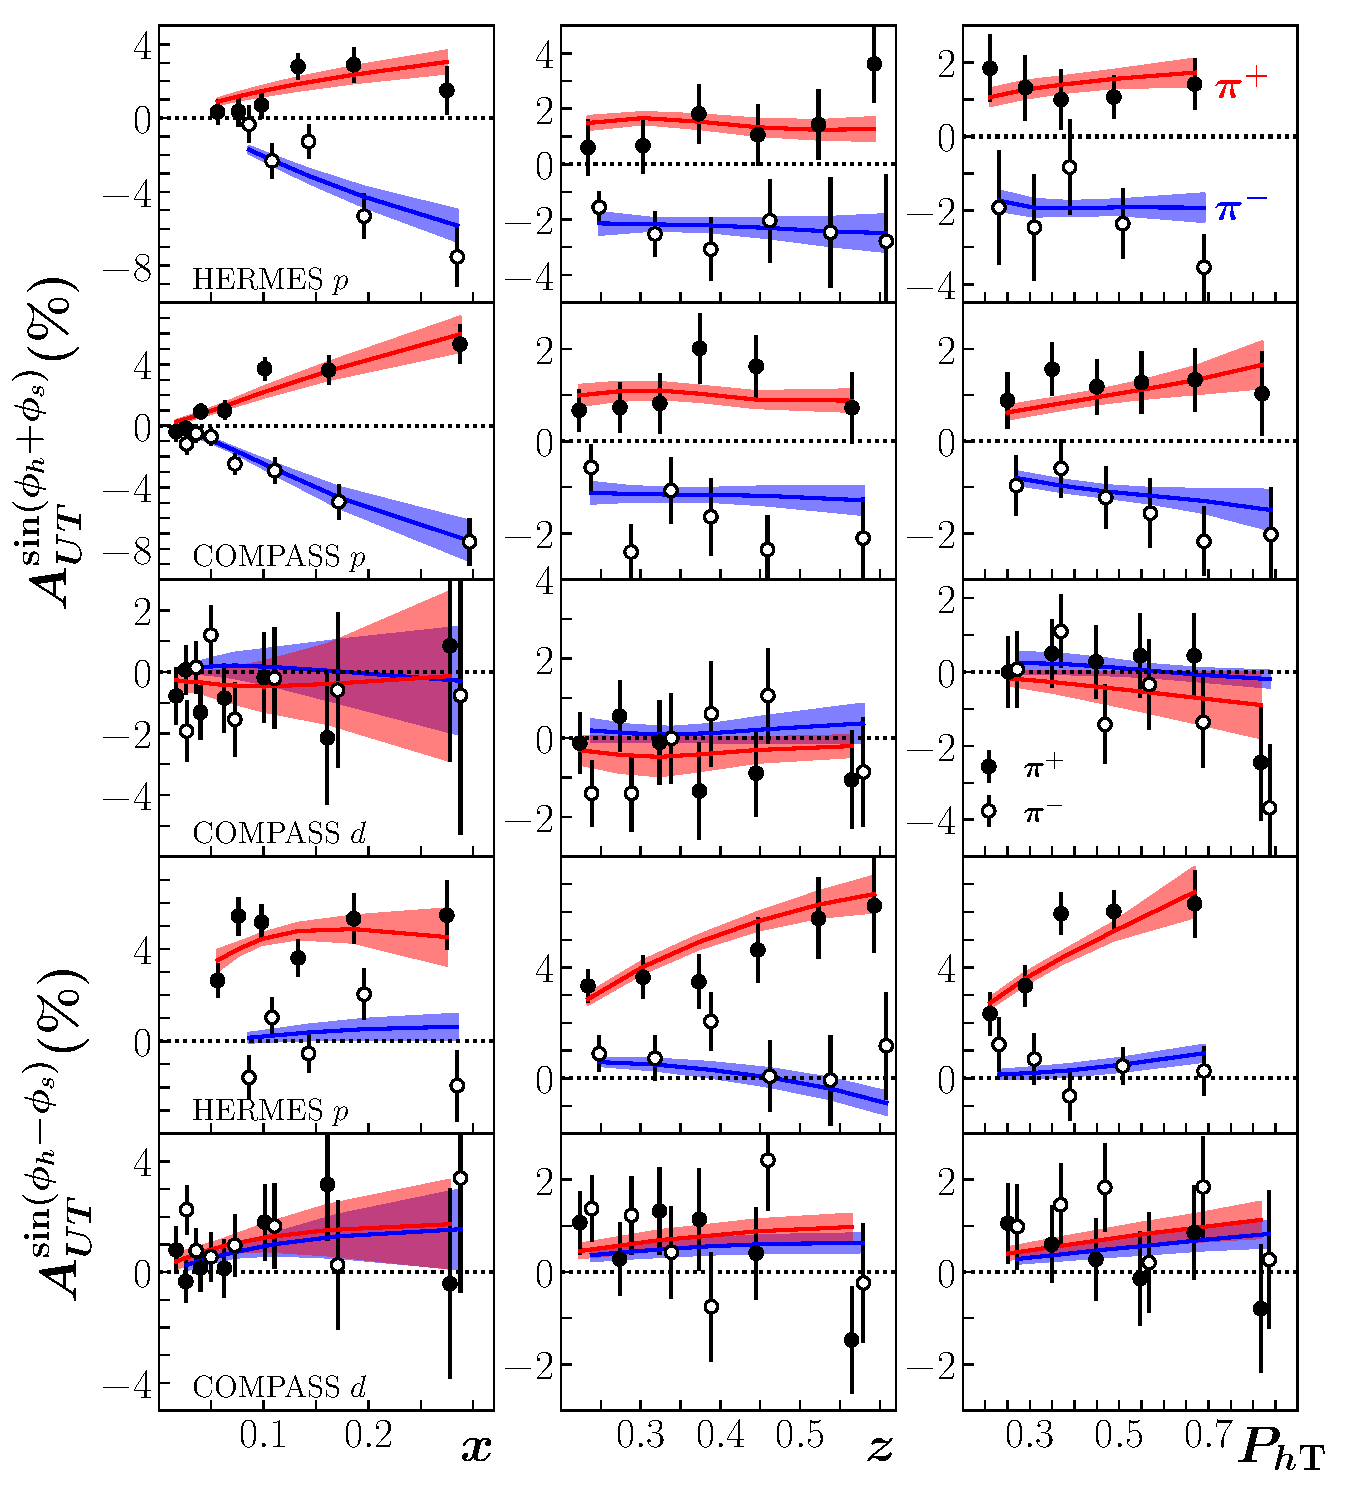
\includegraphics[width=0.5\textwidth]{gallery2/sidis.pdf}
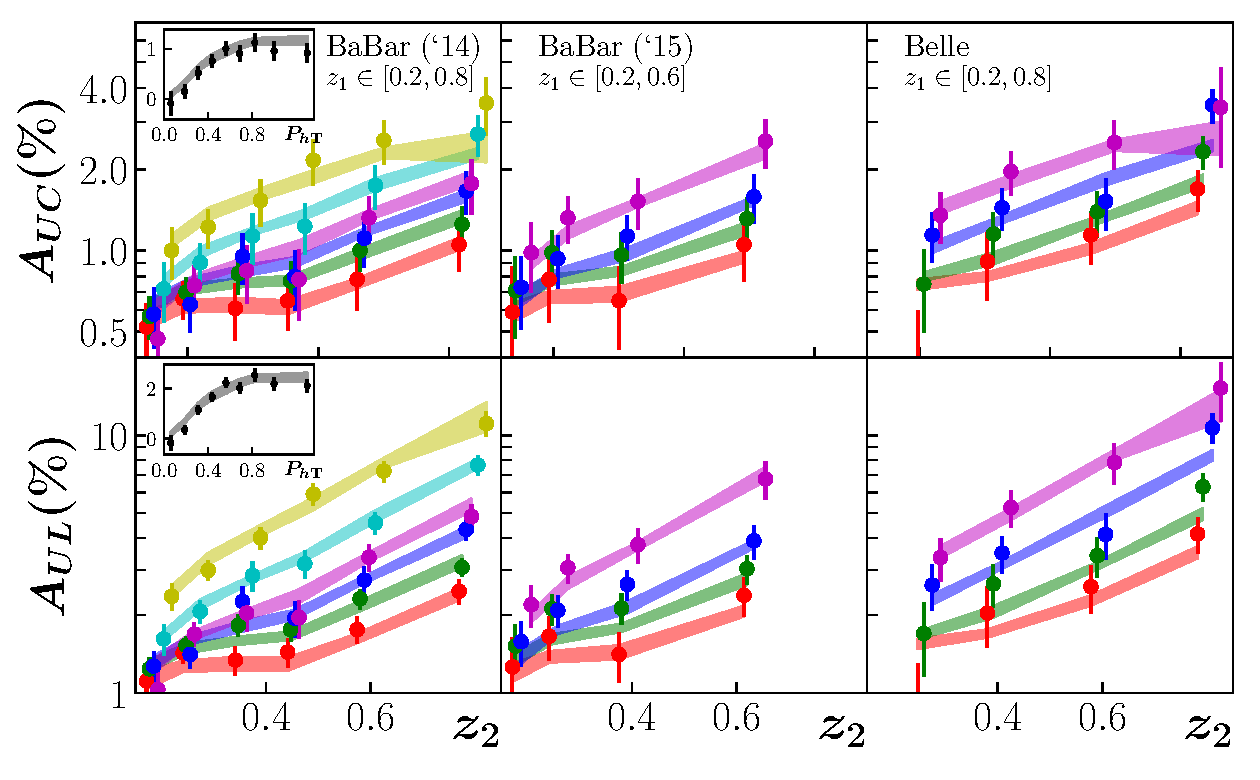
\includegraphics[width=0.5\textwidth]{gallery2/sia.pdf}
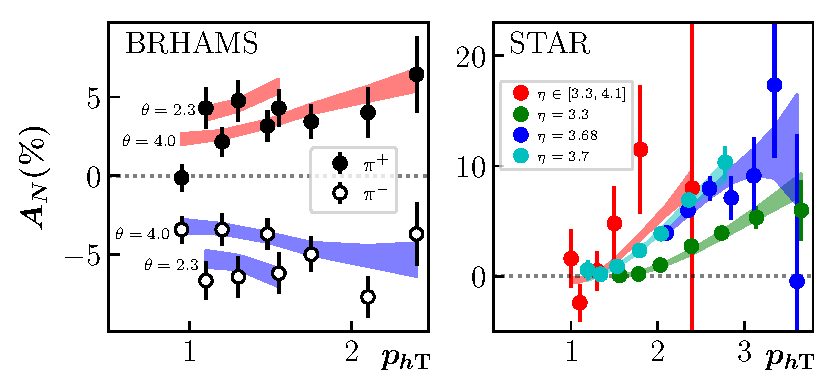
\includegraphics[width=0.5\textwidth]{gallery2/an.pdf}
\caption{.} 
\label{f:SIDIS_Sivers}
\end{figure}

\begin{figure}[h!]
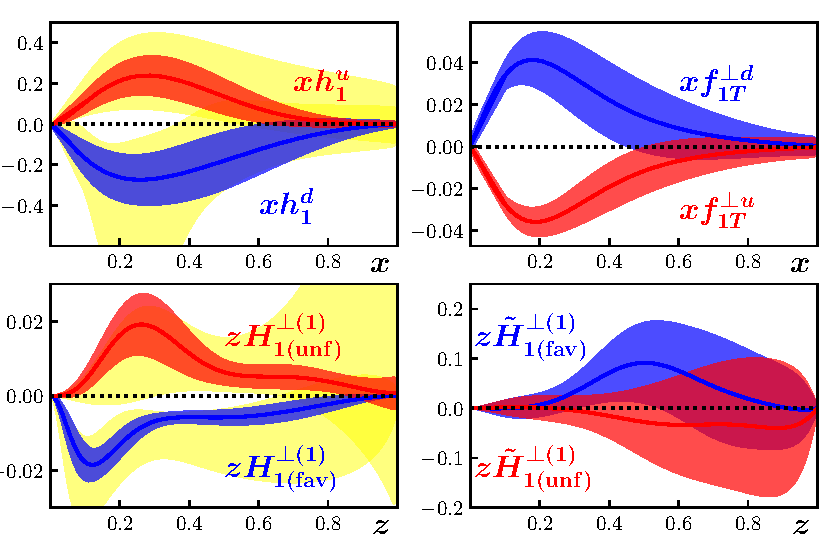
\includegraphics[width=0.5\textwidth]{gallery2/qcf.pdf}
\caption{Extracted functions at $Q^2=42$ GeV$^2$.} 
\label{f:qcf}
\end{figure}

\begin{figure}[h!]
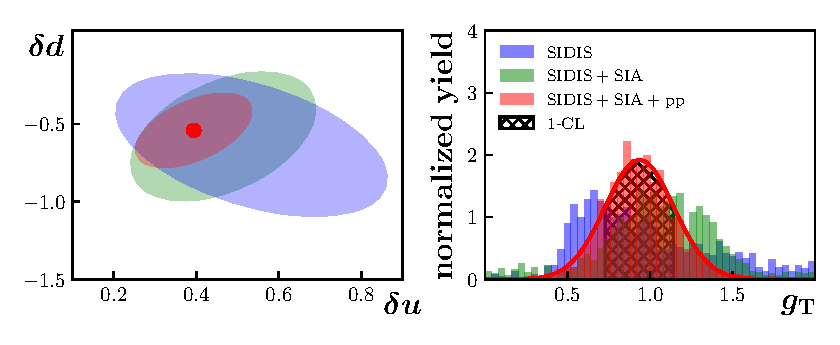
\includegraphics[width=0.5\textwidth]{gallery2/gT.pdf}
\caption{Extracted tensor charge at $Q^2=42$ GeV$^2$.} 
\label{f:gT}
\end{figure}


%%%%%%%%%%%%%%%%%%%%%%%%%%%%%%%%%%%%%%%%%%%%%%%%%%%%%%%%%%%%%%%%%%%%
\vspace{0.1cm}
\noindent {\it \bf Conclusions.} 
%
In this paper we have shown for the first time through phenomenology
that SSAs in a variety of processes have a common origin.  
%
Namely, they are due to the intrinsic quantum-mechanical interference
of multi-parton states. 
%
We have performed the first global analysis of the available
experimental SSA data in SIDIS, DY, $e^+e^-$, and proton-proton
collisions. 

%The extracted set of TMDs and twist-3 functions are compatible with
%previous extractions that separately studied SSAs sensitive TMDs or
%SSAs involving collinear twist-3 functions.  the previous separate
%global fit results and is compatible, albeit a 1-$\sigma$ tension
%with $u$-quark tensor charge, with lattice QCD results.
The future data from Jefferson Lab 12 GeV, an upgraded RHIC, and the
Electron-Ion Collider will help to reduce the uncertainties of the
extracted functions and ultimately will lead to the better
understanding of the structure of hadrons, including gluon and
antiquark functions.
%
The future development of our study will include inclusion of complete
QCD evolution, and data sets from other facilities, such as LHC.

%%%%%%%%%%%%%%%%%%%%%%%%%%%%%%%%%%%%%%%%%%%%%%%%%%%%%%%%%%%%%%%%%%%%
\vspace{0.1cm}
\noindent {\it \bf Ackowledgments.}  
This paper was supported in part by the National Science Foundation under Grant No.~PHY-1623454 (A.P.), No.~PHY-1720486 (Z.K.), the DOE Contracts DOE Contract No. DE- AC05-06OR23177 (L.G.) and No.~DE- AC05-06OR23177 (A.P., N.S.), under which Jefferson Science Associates, LLC operates Jefferson Lab. This work is also supported within the framework of the TMD Topical
Collaboration.

The work of J.A.M.~and D.P.~has been partially supported by a Lebanon
Valley College Edward H. Arnold and Jeanne Donlevy Arnold
Student-Faculty Research Grant.

%\appendix
%\section{Complementary material}

\bibliography{dp}

\end{document}


%%%%%%%%%%%%%%%%%%%%%%%%%%%%%%%%%%%%%%%%%%%%%%%%%%%%%%%%%%%%%%%%%%%%
%%%%%%%%%%%%%%%%%%%%%%%%%%%%%%%%%%%%%%%%%%%%%%%%%%%%%%%%%%%%%%%%%%%%
%%%%%%%%%%%%%%%%%%%%%%%%%%%%%%%%%%%%%%%%%%%%%%%%%%%%%%%%%%%%%%%%%%%%
%%%%%%%%%%%%%%%%%%%%%%%%%%%%%%%%%%%%%%%%%%%%%%%%%%%%%%%%%%%%%%%%%%%%


%%%%%%%%%%%%%%%%
%\begin{figure}[h!]
%\centering 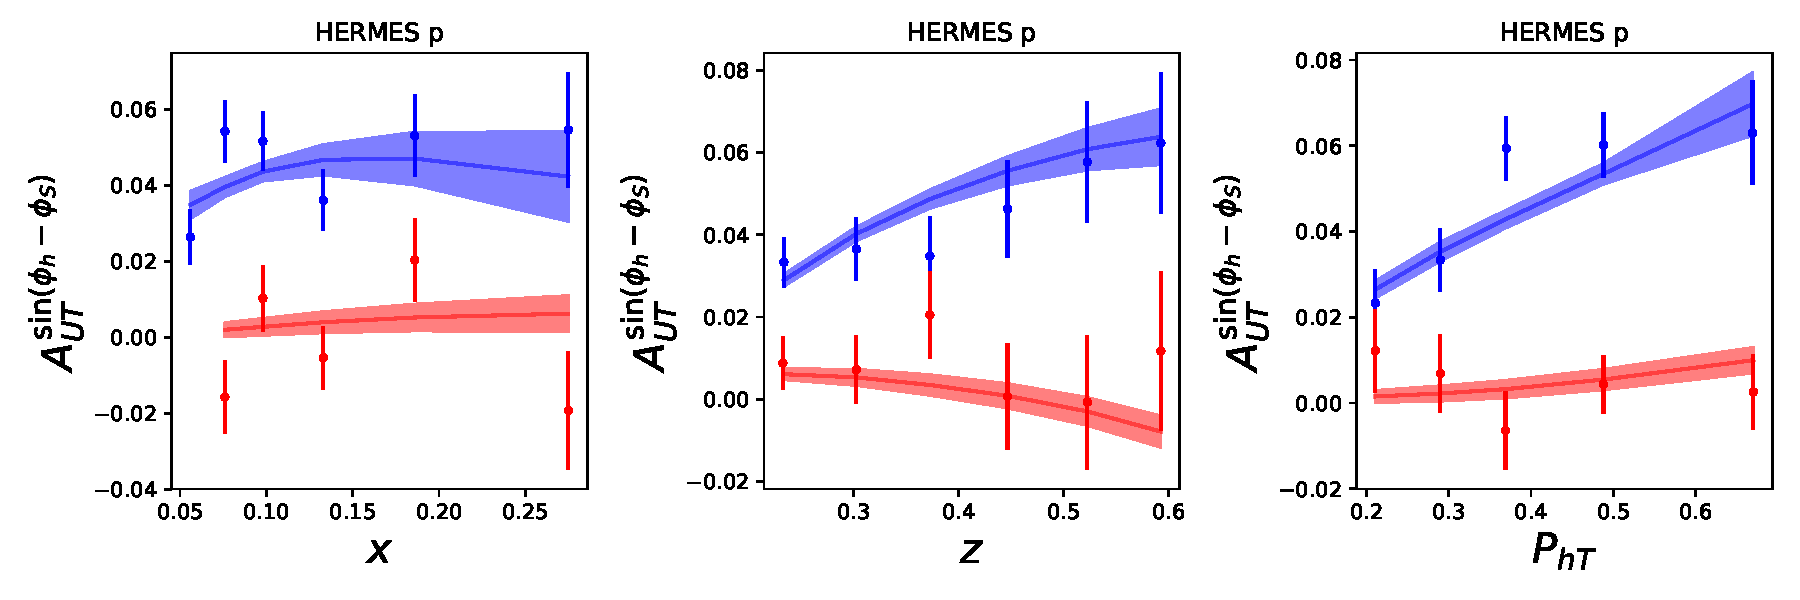
\includegraphics[scale=0.275]{gallery/HERMES_Sivers.pdf}\\
%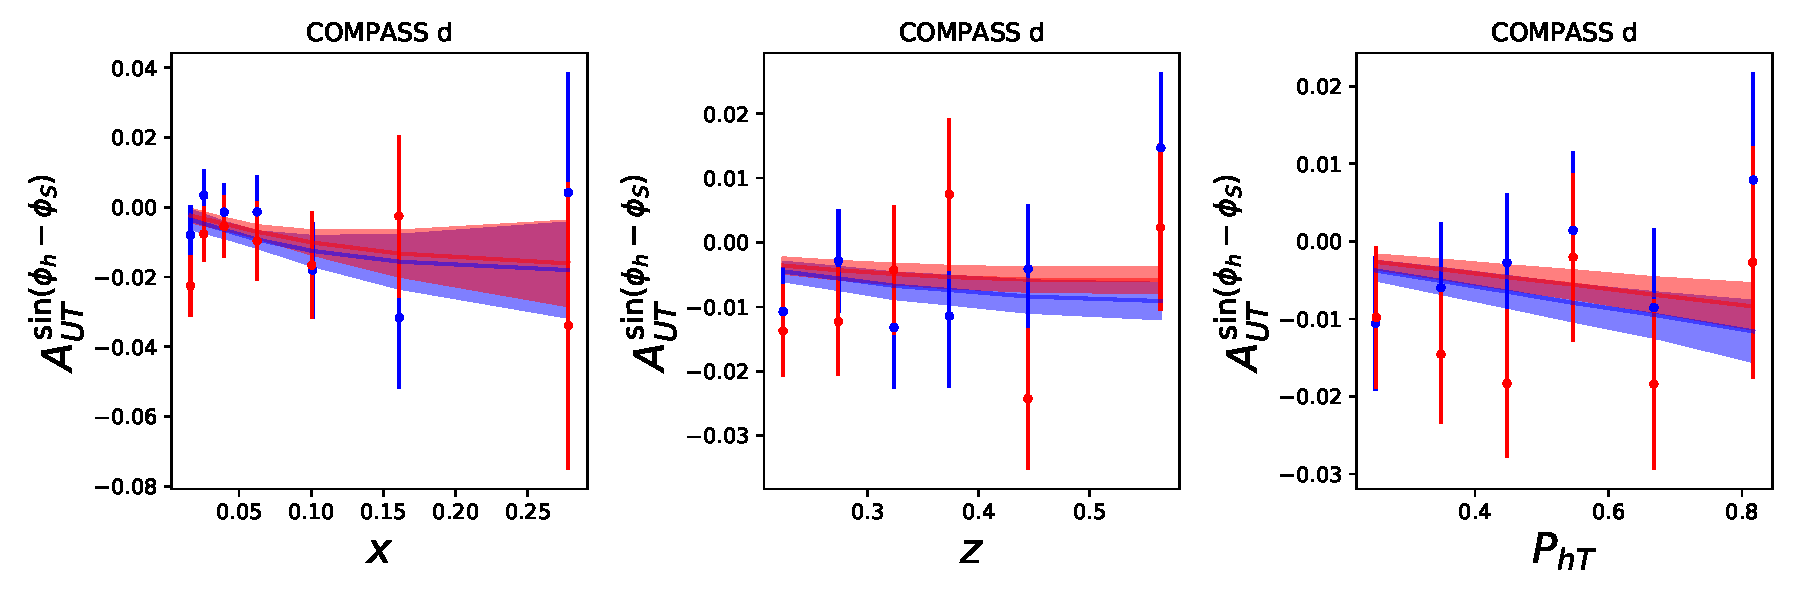
\includegraphics[scale=0.275]{gallery/COMPASS_Sivers.pdf}
%\caption{Results of our global fit compared to Sivers effect data from HERMES and COMPASS.} \label{f:SIDIS_Sivers}
%\end{figure}
%%%%%%%%%%%%%%%%

%%%%%%%%%%%%%%%%
%\begin{figure}[h!]
%\centering 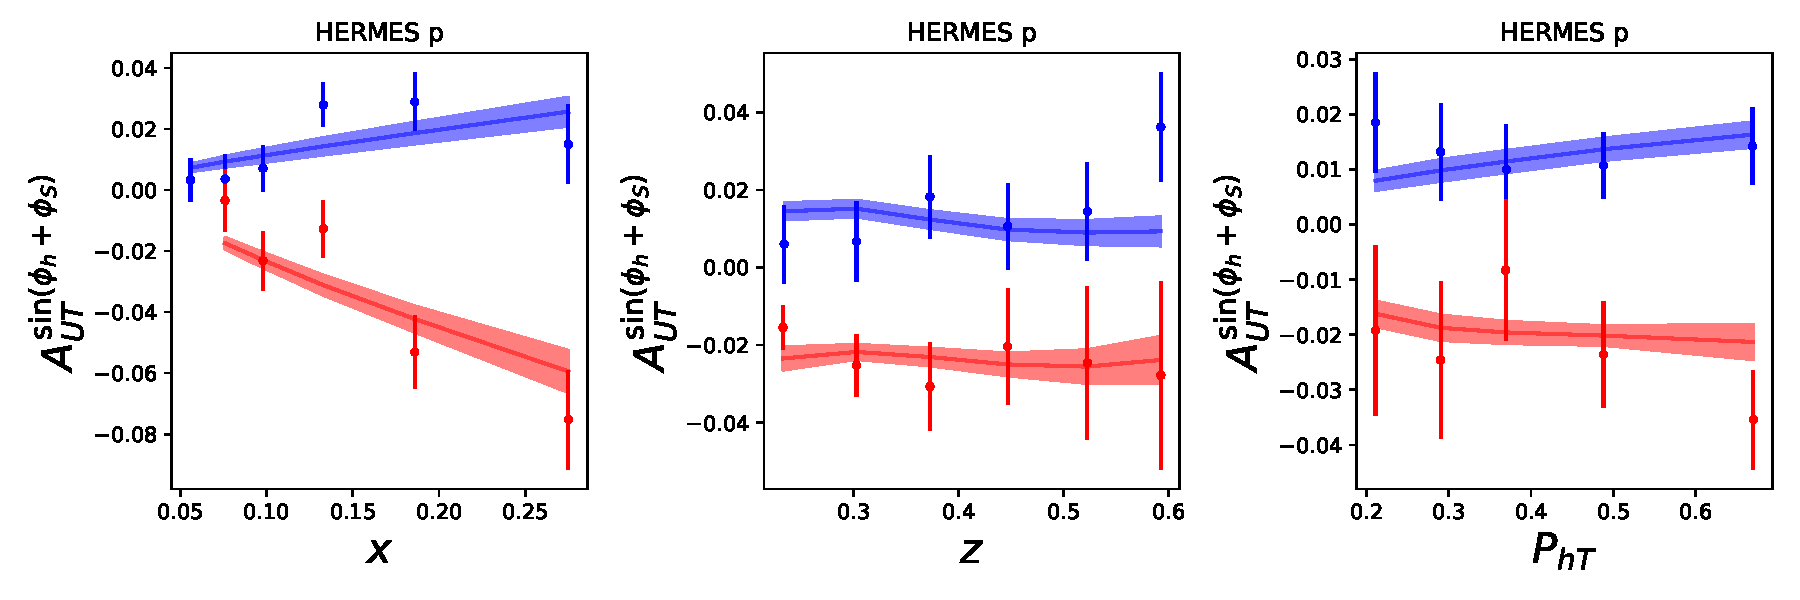
\includegraphics[scale=0.275]{gallery/HERMES_Collins.pdf} \\
%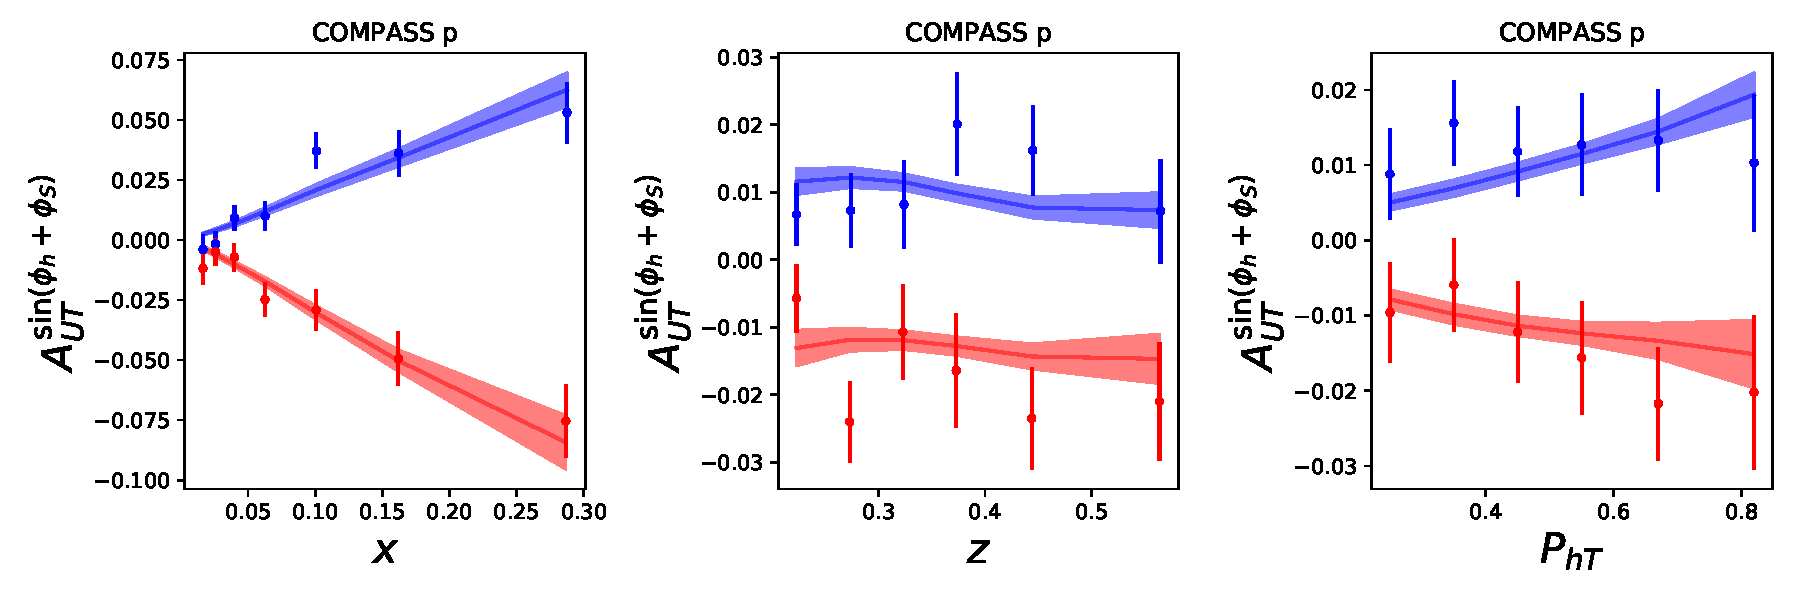
\includegraphics[scale=0.275]{gallery/COMPASS_Collins.pdf} \\
%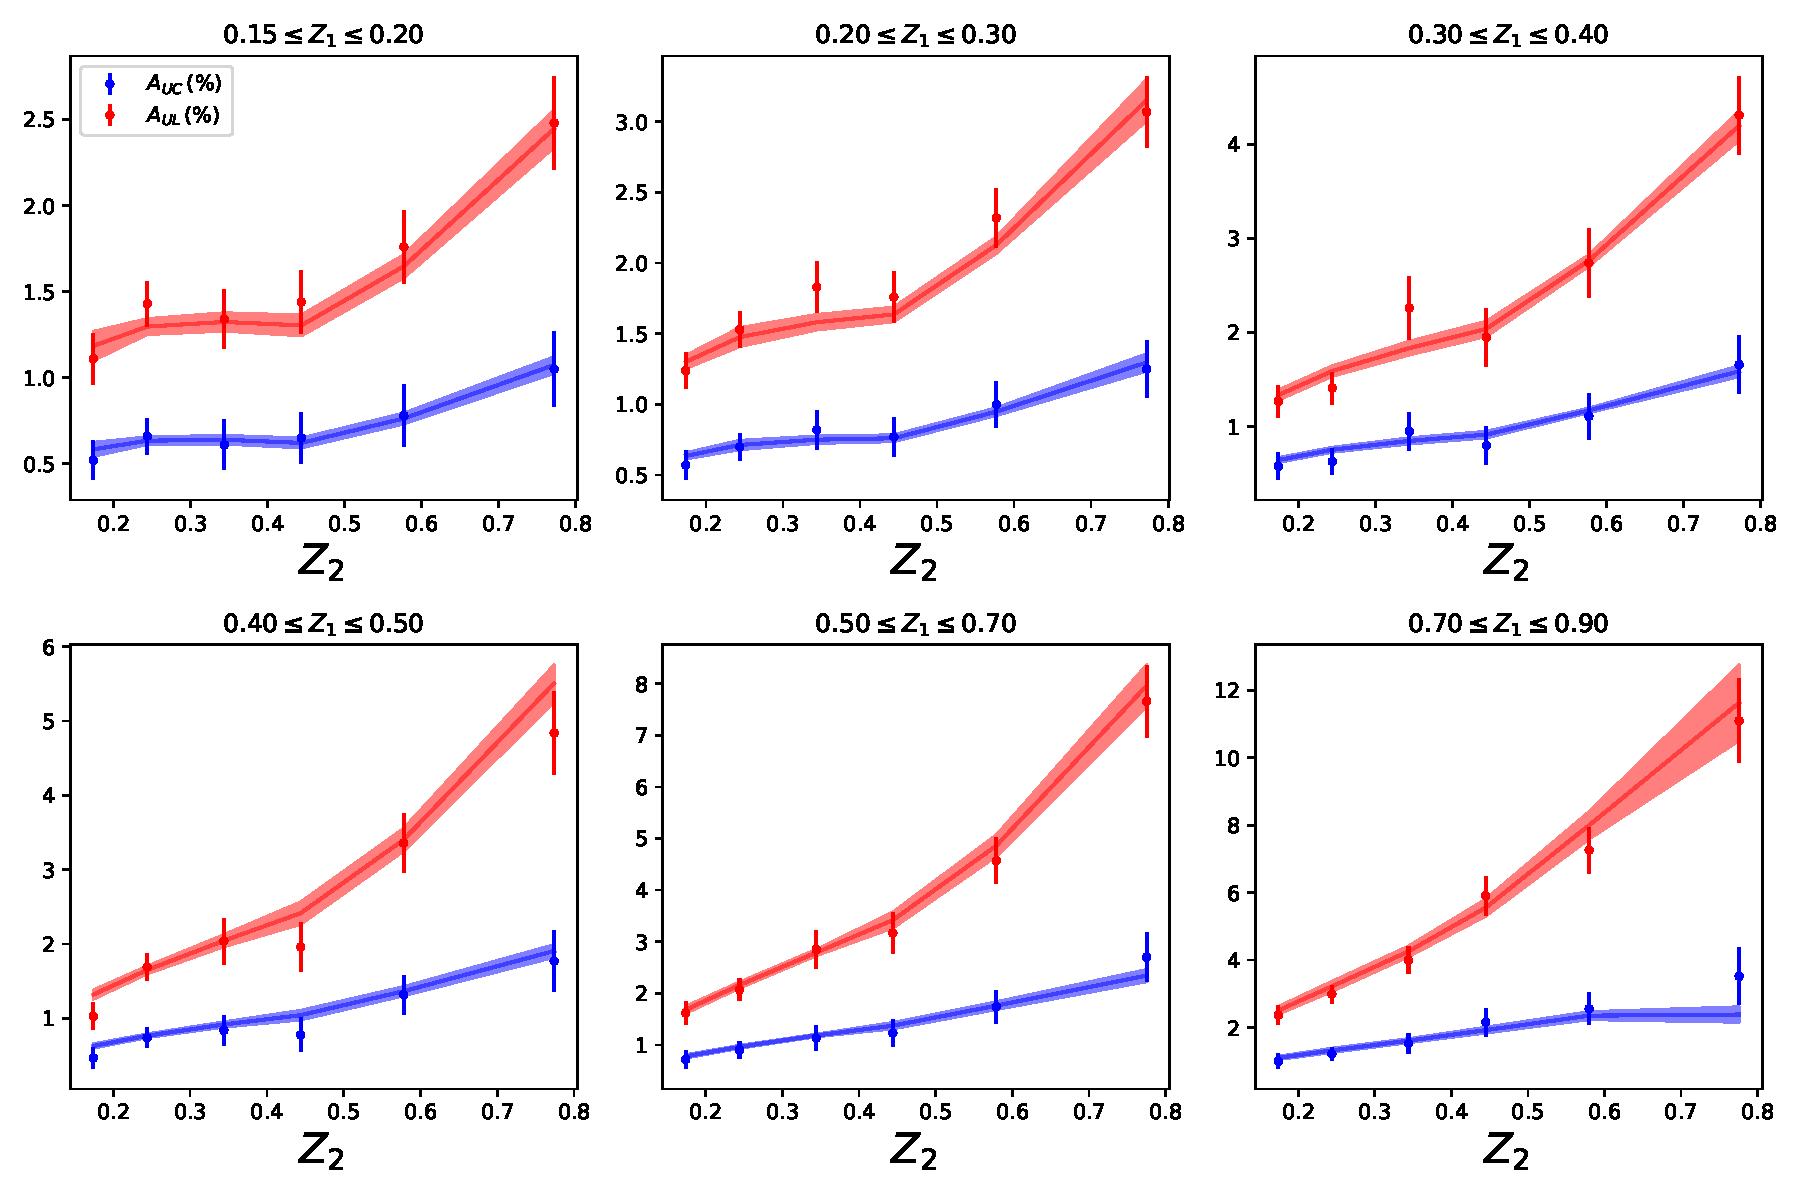
\includegraphics[scale=0.25]{gallery/BaBar_SIA.pdf} \\
%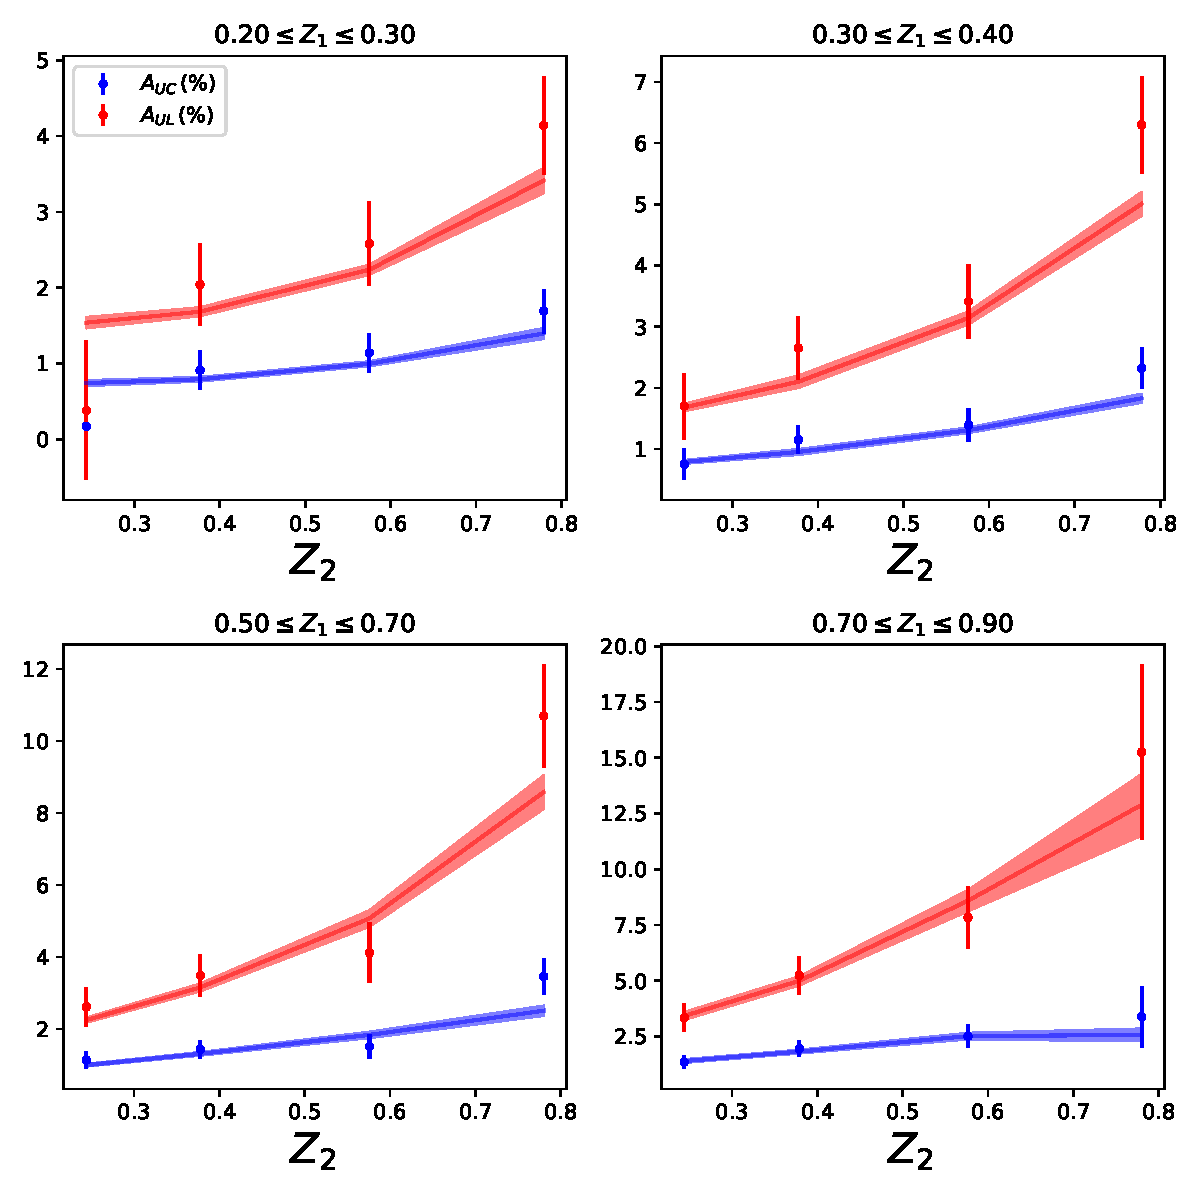
\includegraphics[scale=0.3]{gallery/BELLE_SIA.pdf} 
%\caption{Results of our global fit compared to Collins effects data in SIDIS from HERMES and COMPASS, and in SIA from BaBar and Belle.} \label{f:SIDIS_SIA_Collins}
%\end{figure}
%%%%%%%%%%%%%%%%

%%%%%%%%%%%%%%%%
%\begin{figure}[h!]
%\centering 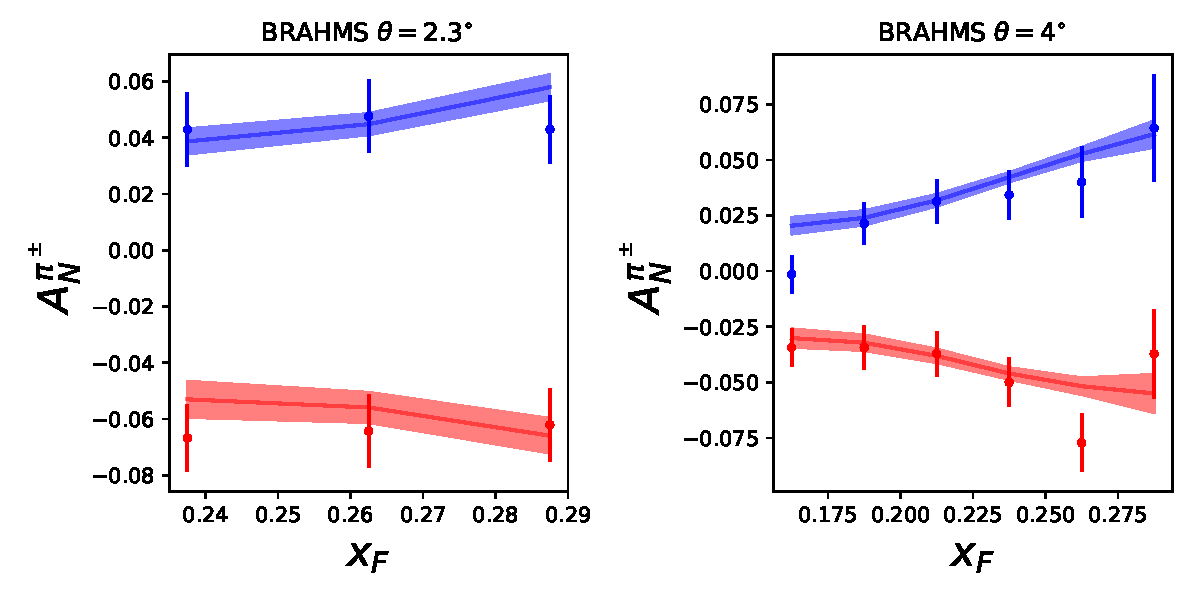
\includegraphics[scale=0.35]{gallery/AN_BRAHMS.pdf}\\
%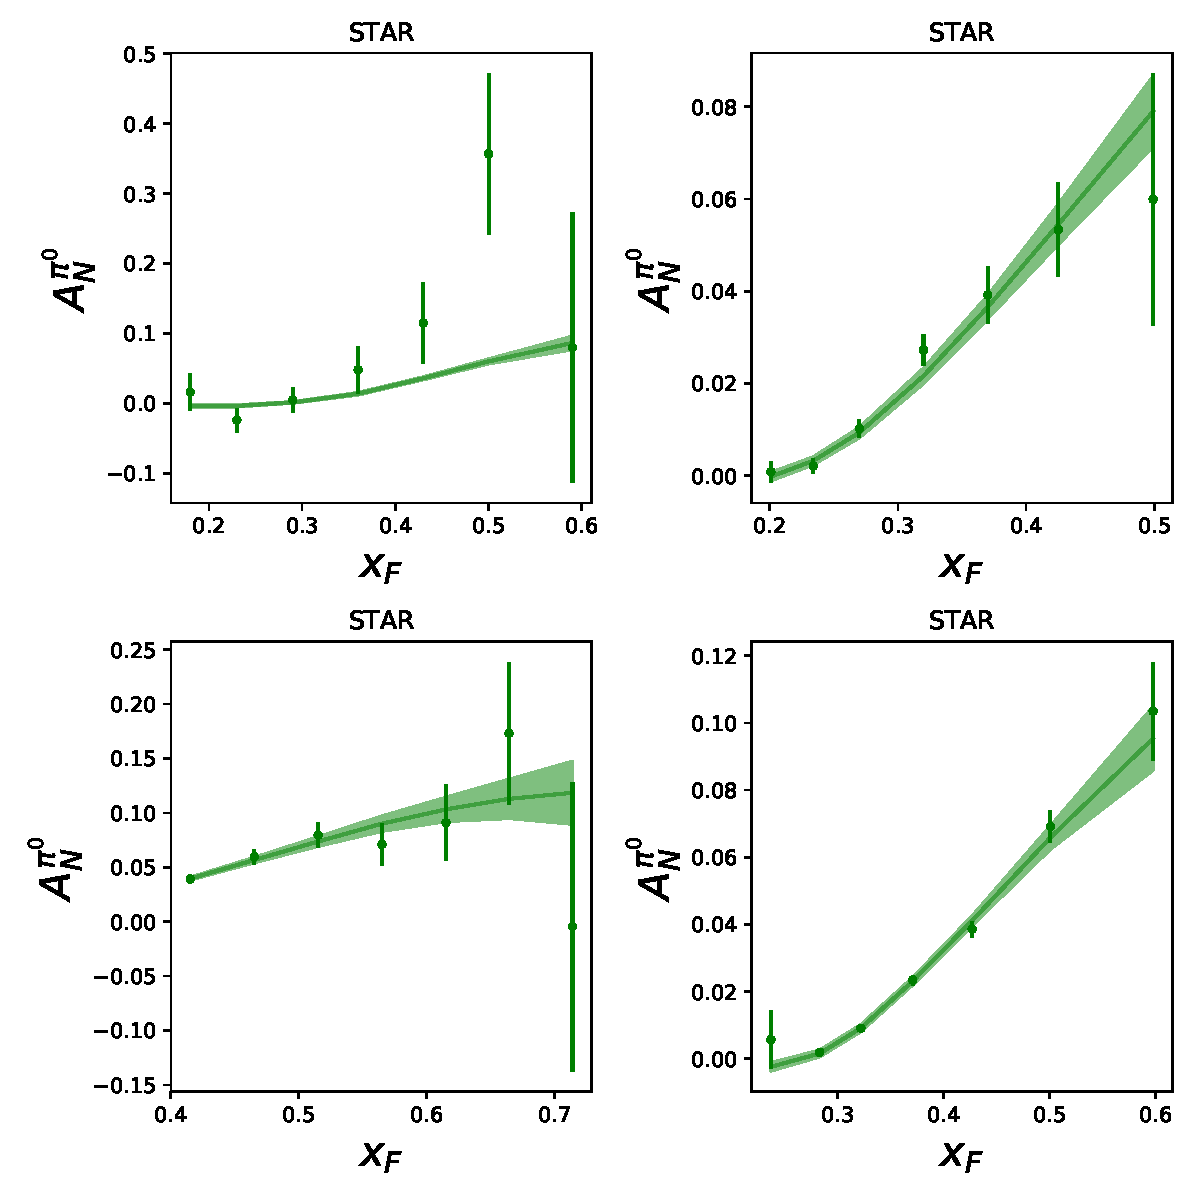
\includegraphics[scale=0.35]{gallery/AN_STAR.pdf} 
%\caption{Results of our global fit compared to $A_N$ data from BRAHMS and STAR.} \label{f:SIDIS_SIA}
%\end{figure}
%%%%%%%%%%%%%%%%

%%%%%%%%%%%%%%%%
%\begin{figure}[h!]
%\centering 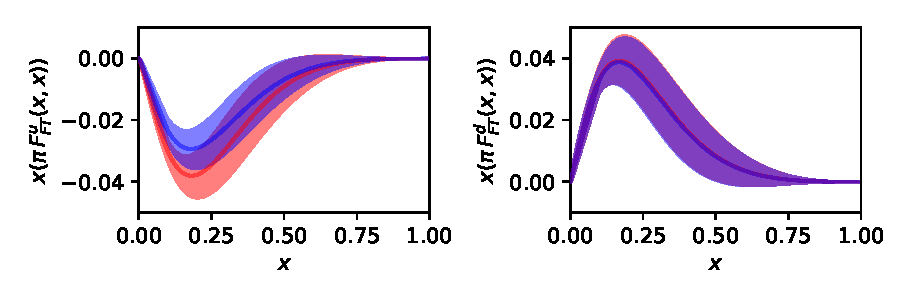
\includegraphics[scale=0.535]{gallery/sivers.pdf}\\
%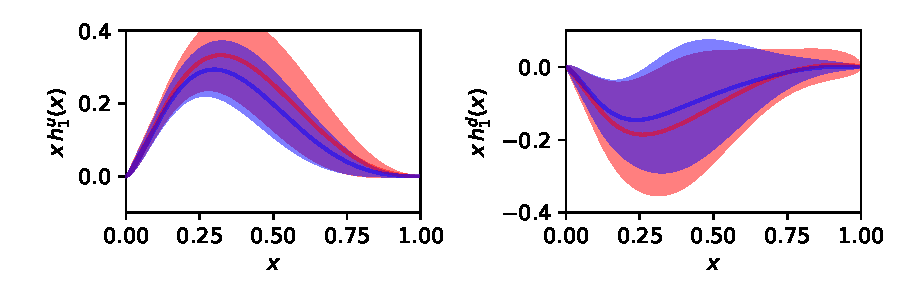
\includegraphics[scale=0.55]{gallery/transversity.pdf}\\
%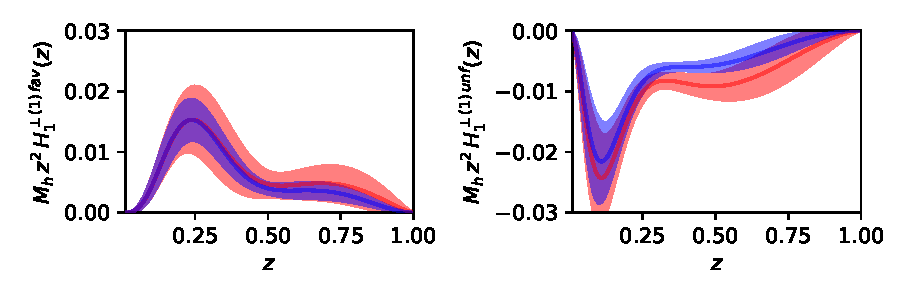
\includegraphics[scale=0.55]{gallery/collinspi.pdf}\\
%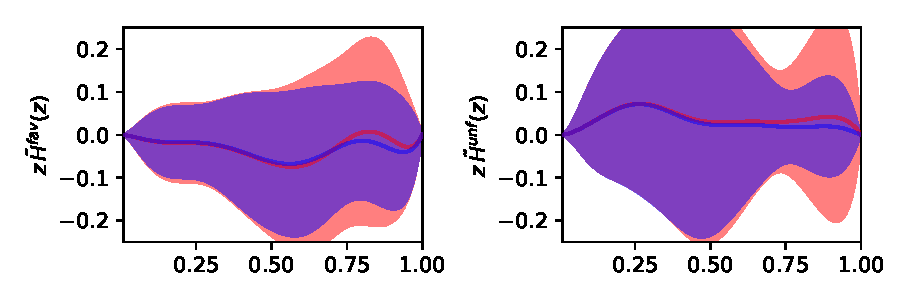
\includegraphics[scale=0.545]{gallery/Htildepi.pdf}\\
%\caption{Extraction of $F_{FT}(x,x)$, $h_1(x)$, $H_1^{\perp(1)}$, and $\tilde{H}(z)$.} \label{f:functions}
%\end{figure}
%%%%%%%%%%%%%%%%

%%%%%%%%%%%%%%%%
%\begin{figure}[h!]
%\centering 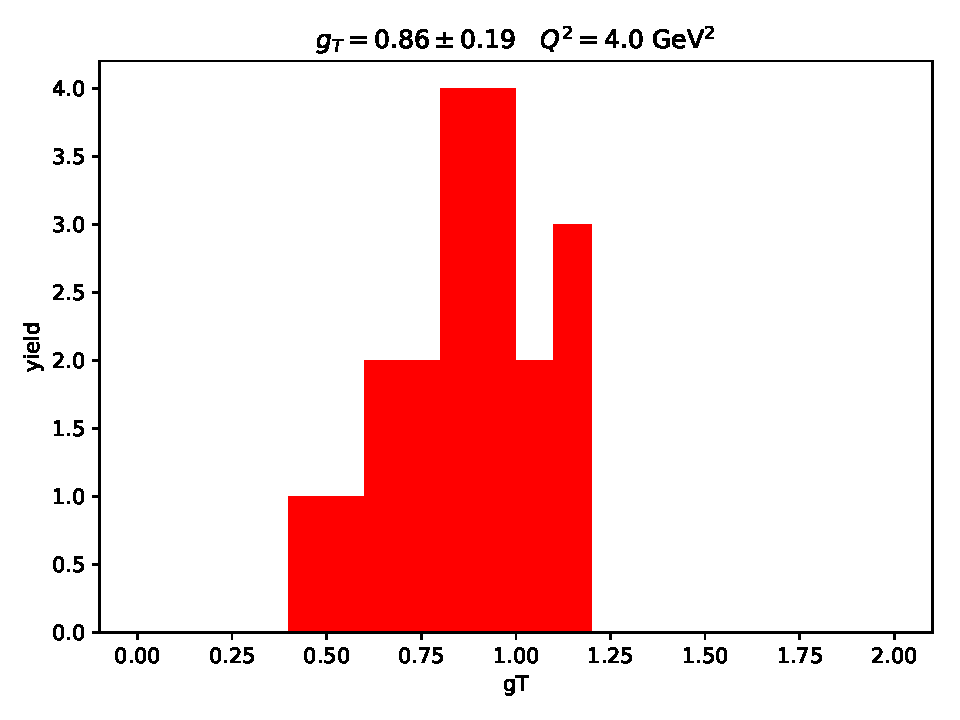
\includegraphics[scale=0.535]{gallery/gT.pdf}\\
%\caption{Tensor charge using our transversity function.} \label{f:tensor}
%\end{figure}
%%%%%%%%%%%%%%%%
